%%\chapter{\textit{Python}}%%

Pada Ba ini akan di bahas cara atau langkah langkah dari penggunaan sistem, yang di mulai dari proses login sistem kemudian memilih menu kelola user atau user pada dashboard admin, selanjutnya menambhkan user yang dapat melakukan proses entropy, setelah itu masuk ke halaman utama atau dashboard user. kemudian melakukan kelola data alternatif yang di lakukan oleh user pengguna serta perbedaanya dengan yang di lakukan oleh user admin, kemudian dilanjutkan dengan proses entropy yang di lakukan oleh user admin dan user pengguna sistem
\pagebreak

\section{Langkah-langkah Menggunakan Sistem}
	langkah-langkah penggunaan sistem di perlukan agar pembaca memahami alur dari sistem yang di buat sehingga pembuat sistem tau apasaja yang di buat serta hasil dari proses yang telah di buat.
\subsection{login}
	Untuk memulai sistem langkah pertama yaitu melakukan login atau masuk ke dalam sistem, adapun hal hal yang dilakukan pada form login yaitu memasukan username dan password, dikarenakan saat membuat sistem user yang pertama di buat yaitu user admin sehingga sehingga user admin dapat melakukan login.
\begin{figure}[!htbp]
	\centerline{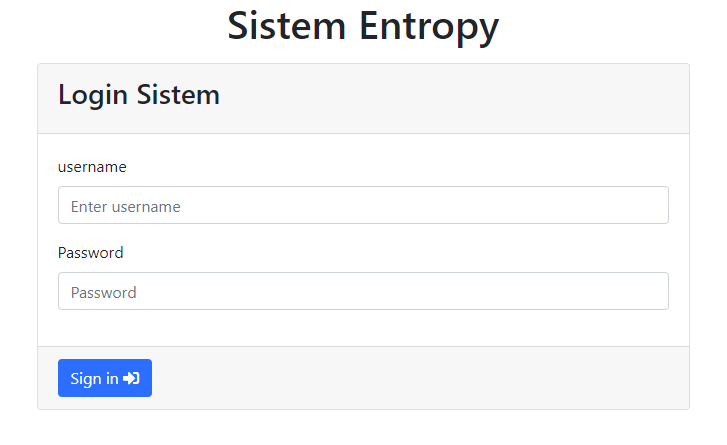
\includegraphics[width=1\textwidth]{figures/view/7.png}}
	\caption{Form Login Sistem}
	\label{l61}
\end{figure}
pada gambar \ref{l61} tersebut merupakan gambar dari form login yang terdiri dari dua form input yaitu input untuk username dan input untuk password. Kemudian jika telah melakukan login terkhusus untuk user admin maka akan muncul tampilan seperti pada gambar \ref{dla6}, pada gambar tersebut user admin memilih menu user, yang bertujuan untuk membuat user pengguna dari sistem ini, untuk proses kelola data user akan di jelaskan pada sub bab kelola data user.
\pagebreak

\begin{figure}[!htbp]
	\centerline{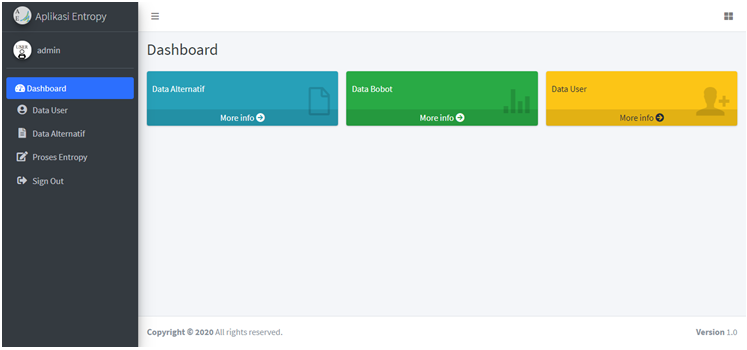
\includegraphics[width=0.90\textwidth]{figures/view/6.png}}
	\caption{view dashboard untuk admin}
	\label{dla6}
\end{figure}

pada gambar \ref{dla6} tersebut merupakan halaman utama untuk user admin atau dashboard untuk admin, halaman ini akan muncul jika user admin melakukan login. kemudian pada halaman utama tersebut terdapat menu data user, data bobot, dan data alternatif.

\begin{figure}[!htbp]
	\centerline{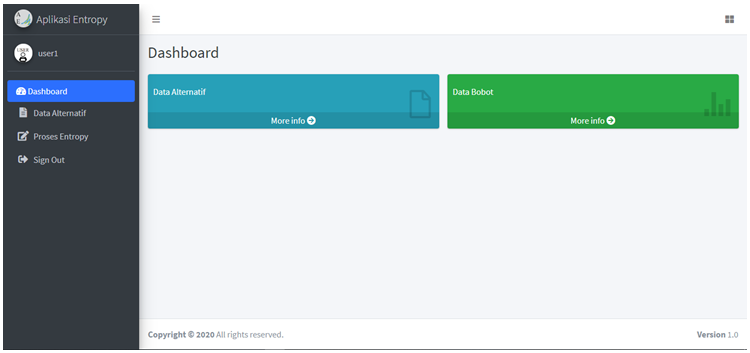
\includegraphics[width=0.90\textwidth]{figures/view/5.png}}
	\caption{view dashboard untuk user}
	\label{dlu6}
\end{figure}

pada gambar \ref{dlu6} merupakan halaman utama untuk user, pada halaman ini hampir sama seperti halaman utama admin hanyasaja satu menu tidak ada yaitu menu kelola data user. emudian untuk memasuki halaman ini user harus melakukan login. hal ini bisa di lakukan jika user admin telah membuatkan user baru untuk user pengguna sistem
\pagebreak
\subsection{Kelola data user}

	Dalam mengelola data user pada sistem ini hanya bisa di lakukan oleh user admin saja, sehingga untuk proses create, update, view, dan delete untuk data user hanya bisa di lakukan oleh admin kemudian untuk tampilan index atau halaman untuk menampilkan data user seperti gambar \ref{us1} berikut ini
\begin{figure}[!htbp]
	\centerline{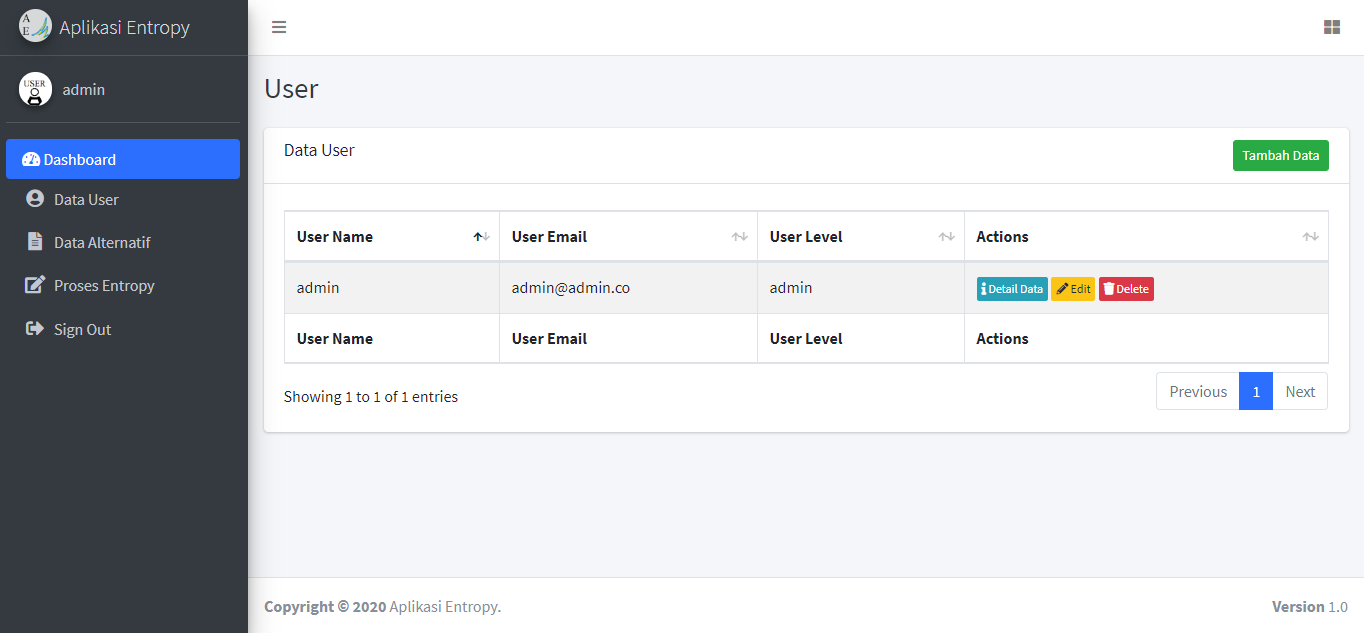
\includegraphics[width=0.90\textwidth]{figures/us1/1.png}}
	\caption{Halaman Data User}
	\label{us1}
\end{figure}
pada gambar \ref{us1} merupakan halaman utama untuk data user, yang mana data user tersebut di simpan dalam bentuk tabel, lalu pada halaman tersebut terdapat empat tombol utama yaitu tombol tambah data, detail data, edit, dan delete, yang mana memiliki fungsinya masing-masing, untuk fungsi setiap tombol tersebut sebagai berikut:
\begin{itemize}
\item tombol tambah data digunakan untuk memanggil halaman tambah data atau form tambah data
\item tombol detail data, di krenakan data setiap user tidak ditampilkan secara keserulurhan maka jika ingin melihat detail data dapat menggunakan tombol ini yang di gunakan untuk berpindah ke halaman detail data dari satu data yang di pilih.
\item tombol edit digunakan untuk memangil halaman edit atau update data 
\item tombol delete, digunakan untuk menghapus data yang telah dipilih
\end{itemize}

kemudian pada tahapan selanjutnya yaitu menambahkan data user yaitu pada halaman tambah data user seperti pada gamabr \ref {us2} pada halaman selanjutnya
\pagebreak
\begin{figure}[!htbp]
	\centerline{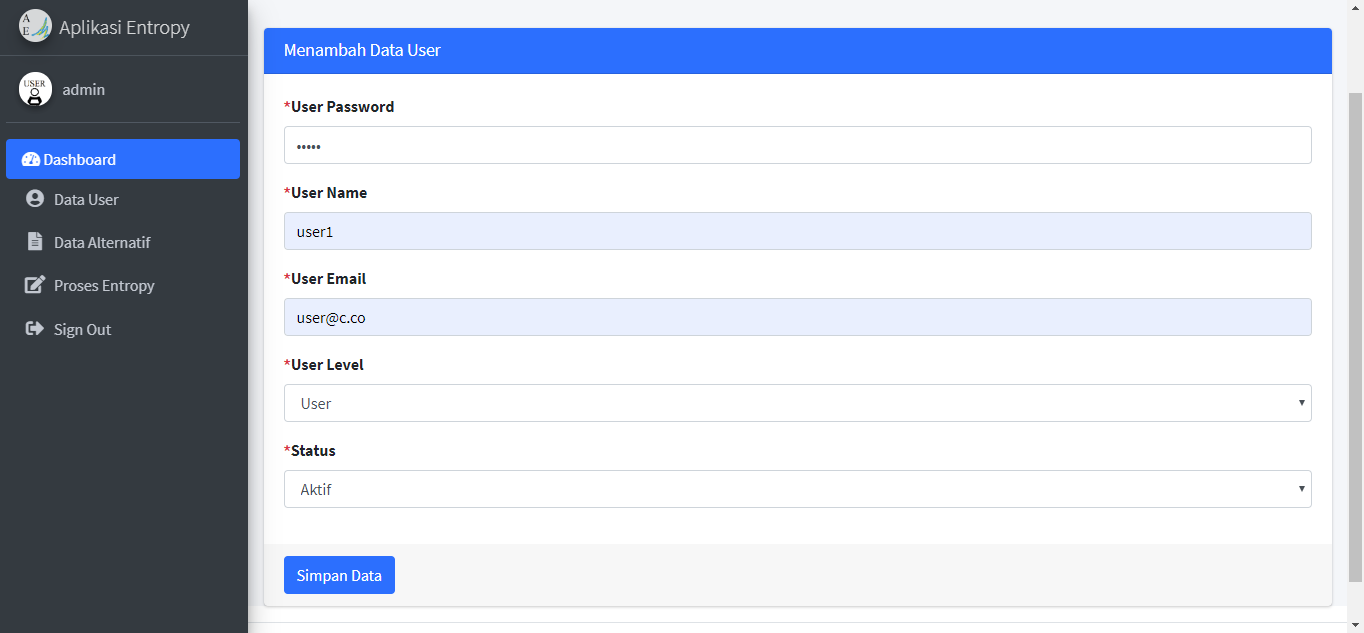
\includegraphics[width=0.90\textwidth]{figures/us1/2.png}}
	\caption{Halaman Tambah Data User}
	\label{us2}
\end{figure}

pada gambar \ref{us2} merupakan form input data user dimana data-data tersebut wajib di isi, adapun data-data yang wajib di isi pada form tersebut meliputi data password, username, user email, user level, dan status dari user tersebut.\par
kemudian jika data telah di tambahkan maka hasilnya seperti pada gambar \ref{us3} berikut ini

\begin{figure}[!htbp]
	\centerline{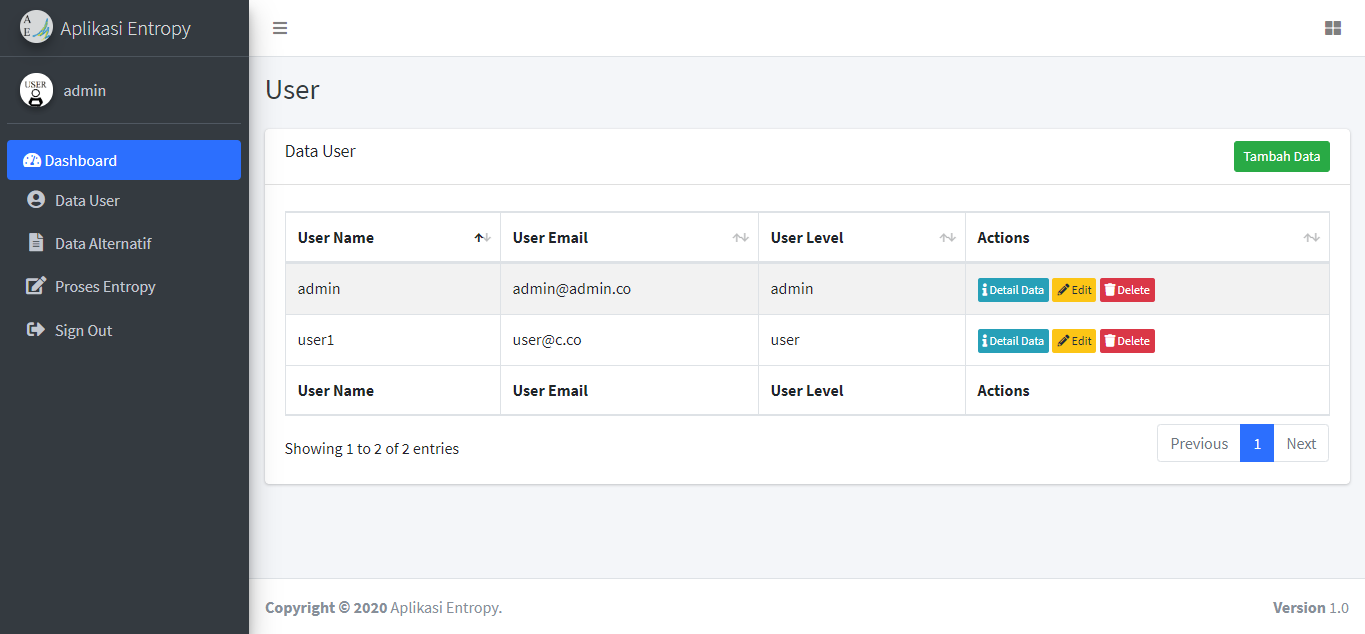
\includegraphics[width=0.90\textwidth]{figures/us1/3.png}}
	\caption{Halaman Data User setelah ditambahkan User baru}
	\label{us3}
\end{figure}
\pagebreak
jika data sudah tersimpan jikalau ada kesalahan dapat melakukan edit data dengan cara masuk ke form edit data seperti pada gambar \ref{us4} berikut ini

\begin{figure}[!htbp]
	\centerline{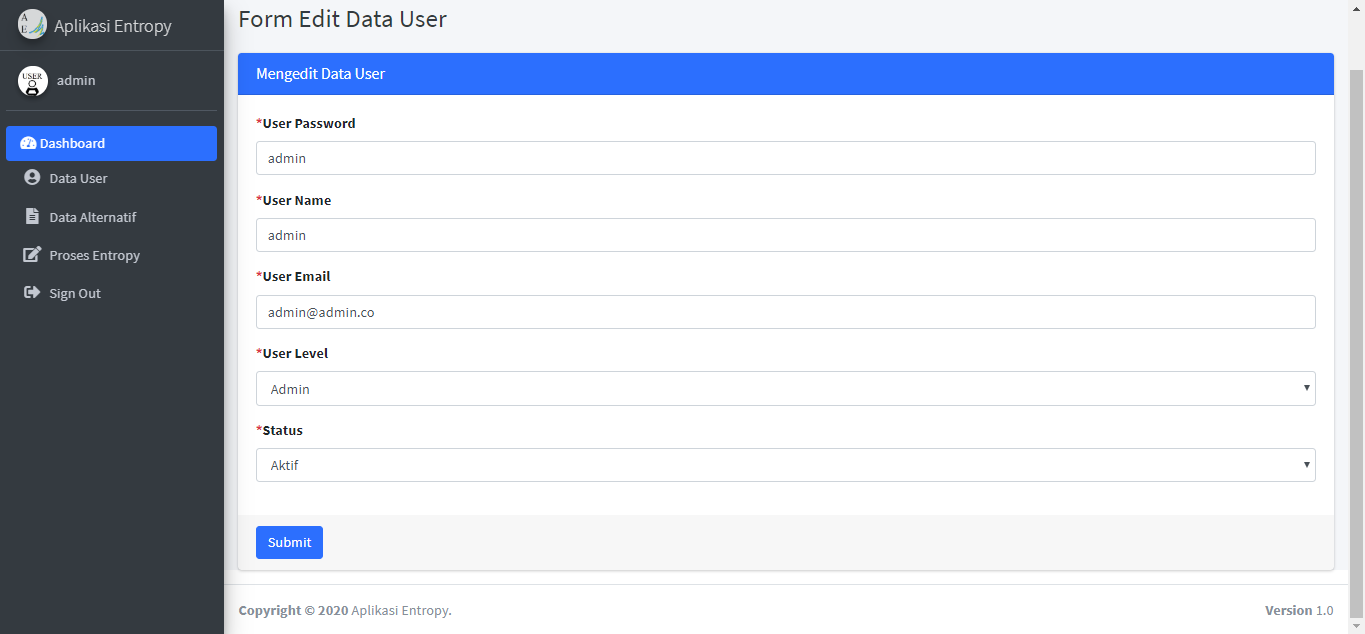
\includegraphics[width=0.90\textwidth]{figures/us1/4.png}}
	\caption{Halaman Edit Data User}
	\label{us4}
\end{figure}

kemudian untuk melihat detail data dari data user dapat melalui tombol detai data maka akan muncul tampilan detail data user seperti pada gambar \ref{us5} berikut

\begin{figure}[!htbp]
	\centerline{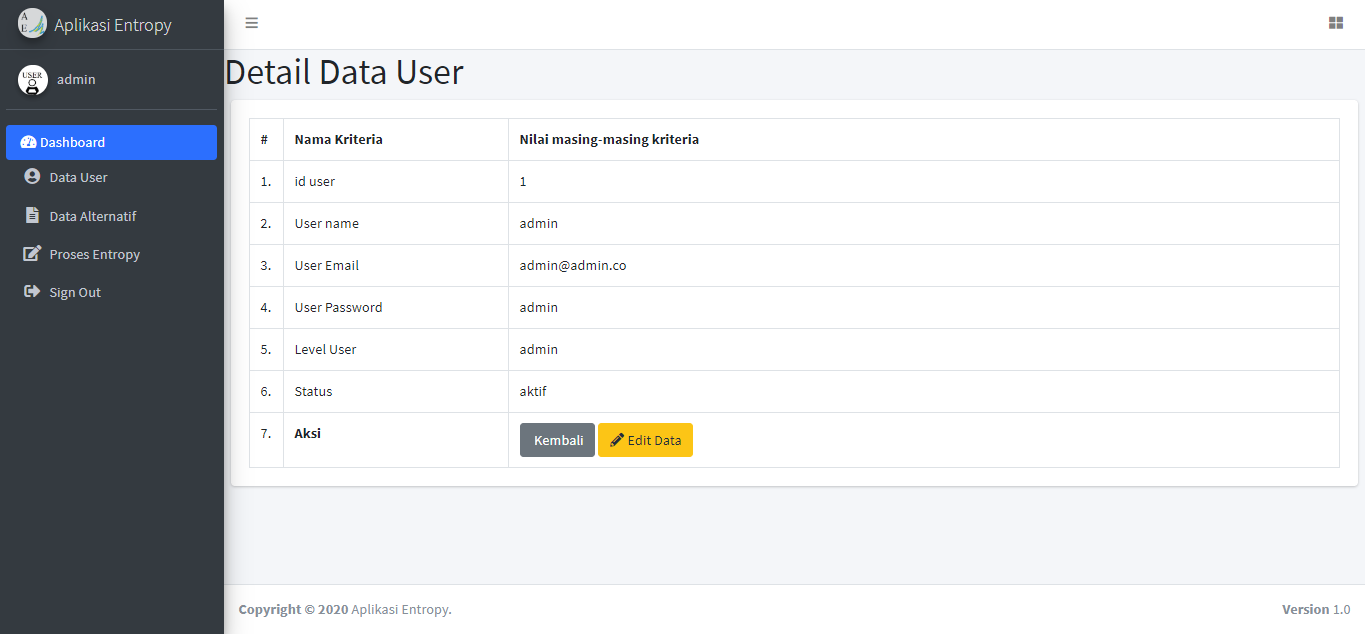
\includegraphics[width=0.90\textwidth]{figures/us1/5.png}}
	\caption{Halaman Detail Data User}
	\label{us5}
\end{figure}

\subsection{Kelola data Alternatif}
	Untuk peroses klola data alternatif dapat di lakukan oleh user admin dan user selain admin atau pengambil bobot, pada halaman utama untuk data alternatif hampir mirip seperti data user, dimana data yang di tampilkan melalui sebuah tabel, kemudian untuk gambar \ref{al1} merupakan tampilan untuk index atau halan utama data alternatif
\pagebreak
\begin{figure}[!htbp]
	\centerline{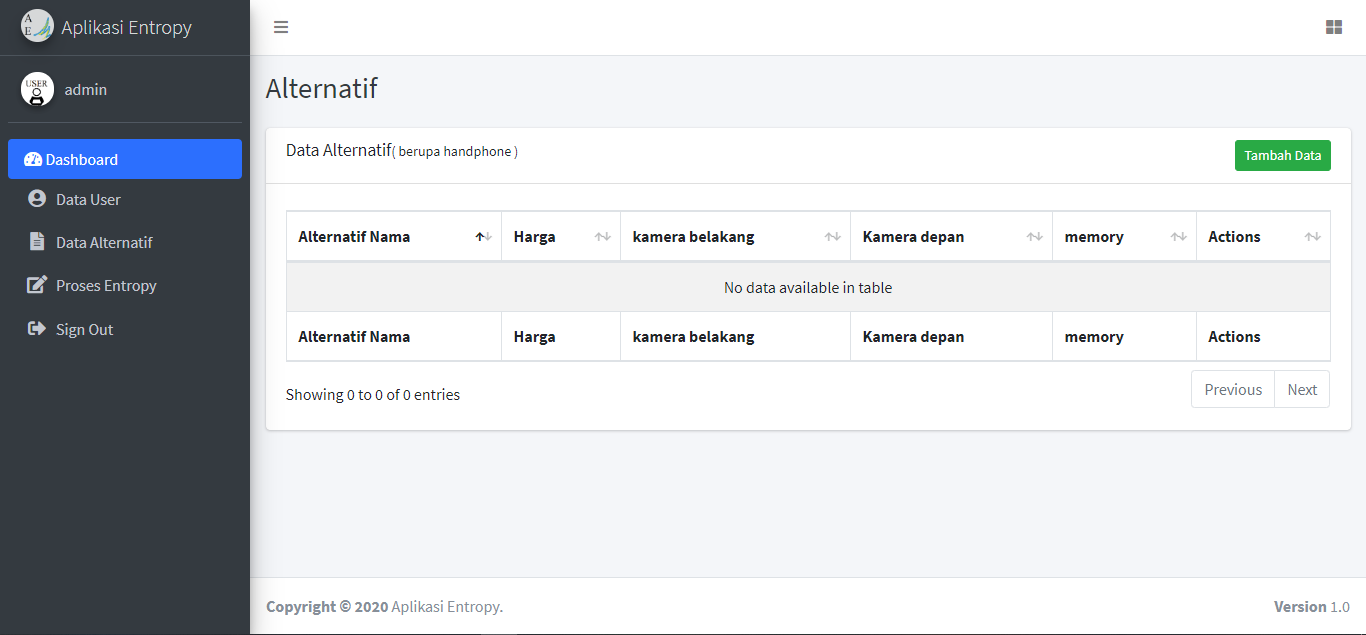
\includegraphics[width=0.90\textwidth]{figures/alte/1.png}}
	\caption{Halaman utama data alternatif}
	\label{al1}
\end{figure}

pada gambar \ref{al1} merupakan halaman utama untuk data alternatif, yang mana data user tersebut di simpan dalam bentuk tabel, lalu pada halaman tersebut terdapat empat tombol utama yaitu tombol tambah data, detail data, edit, dan delete, yang mana memiliki fungsinya masing-masing, untuk fungsi setiap tombol tersebut sebagai berikut:
\begin{itemize}
\item tombol tambah data digunakan untuk memanggil halaman tambah data atau form tambah data
\item tombol detail data, di krenakan data setiap user tidak ditampilkan secara keserulurhan maka jika ingin melihat detail data dapat menggunakan tombol ini yang di gunakan untuk berpindah ke halaman detail data dari satu data yang di pilih.
\item tombol edit digunakan untuk memangil halaman edit atau update data 
\item tombol delete, digunakan untuk menghapus data yang telah dipilih
\end{itemize}
	
\begin{figure}[!htbp]
	\centerline{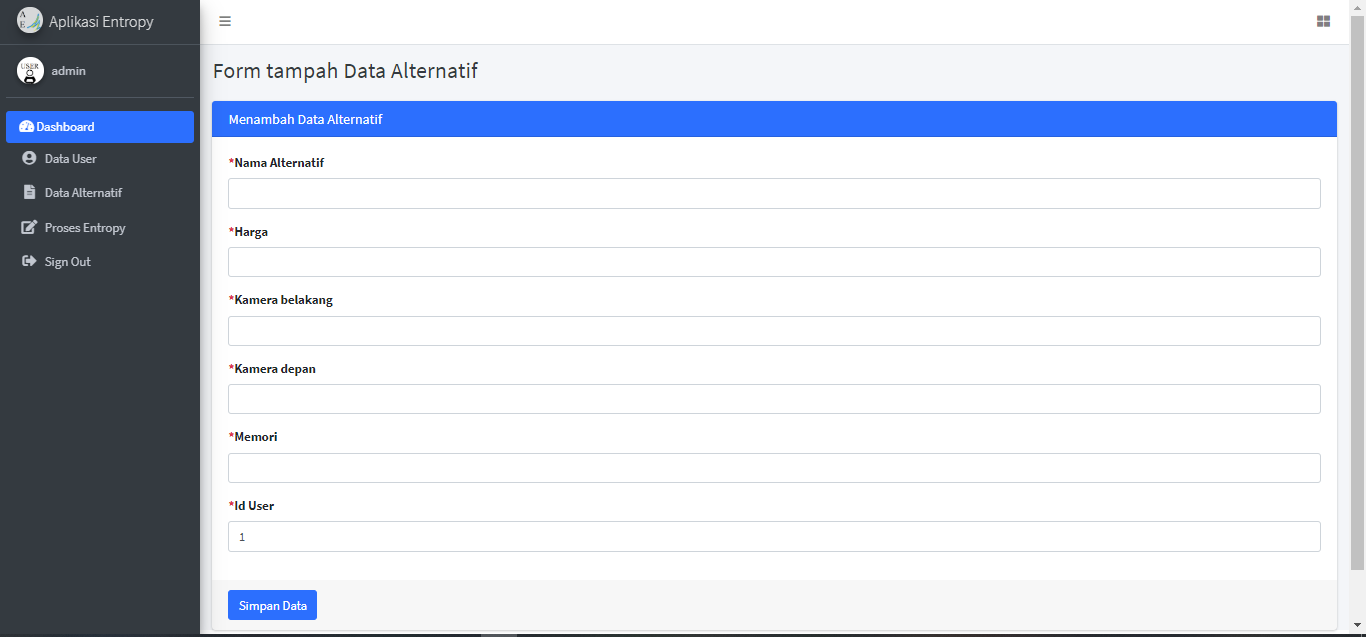
\includegraphics[width=0.90\textwidth]{figures/alte/2.png}}
	\caption{Form tambah data alternatif}
	\label{al2}
\end{figure}
	pada gambar \ref{al2} merupakan form input alternatif, dimana data alternatif wajib di isikan lalu untuk data alternatif yang di isikan yaitu terdiri dari data Nama Alternatif, harga, kamera depan, Memori, kemudian id user akan terisi secara otomatis.
\begin{figure}[!htbp]
	\centerline{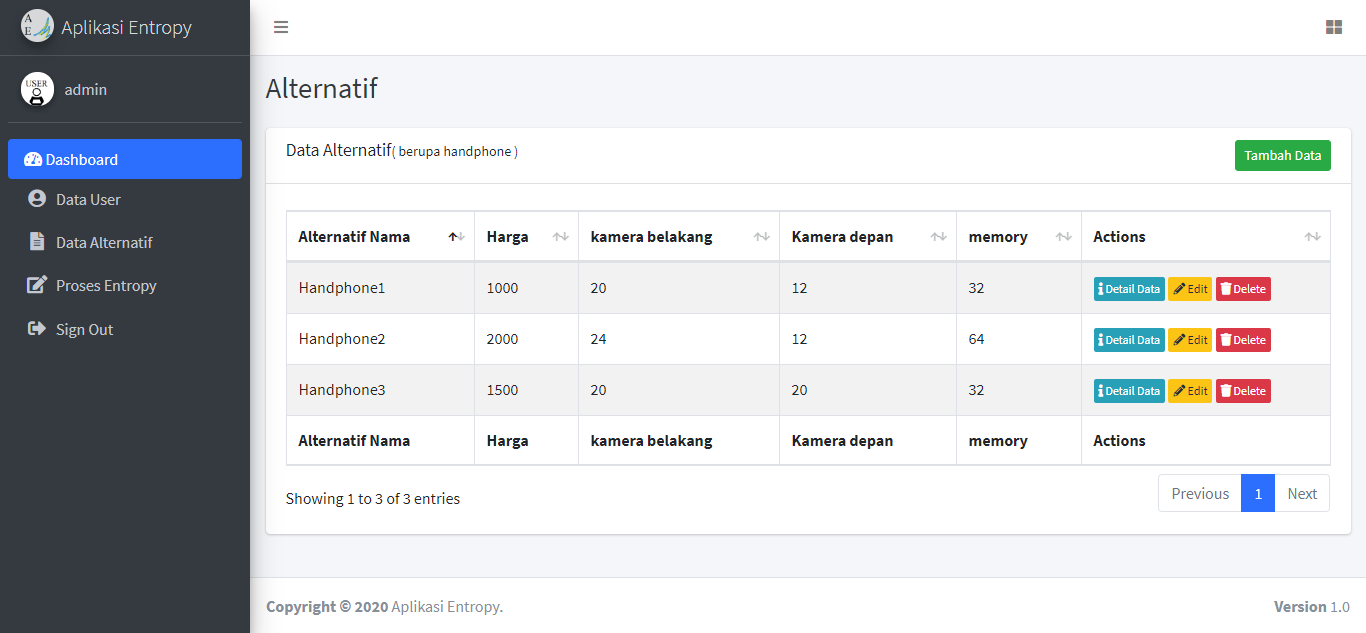
\includegraphics[width=0.90\textwidth]{figures/alte/3.png}}
	\caption{Halaman utama data alternatif setelah ditambah data}
	\label{al3}
\end{figure}
kemudian jika data laternatif telah di tambahkan maka tampilan pada halaman utama untuk data alternatif seperti pada gambar \ref{al3} tersebut. lalu jika ingin mengubah data yang terdapat pada data tersebut dapat menggunakan fitur edit seperti pada gambar \ref{al4} berikut ini.
\begin{figure}[!htbp]
	\centerline{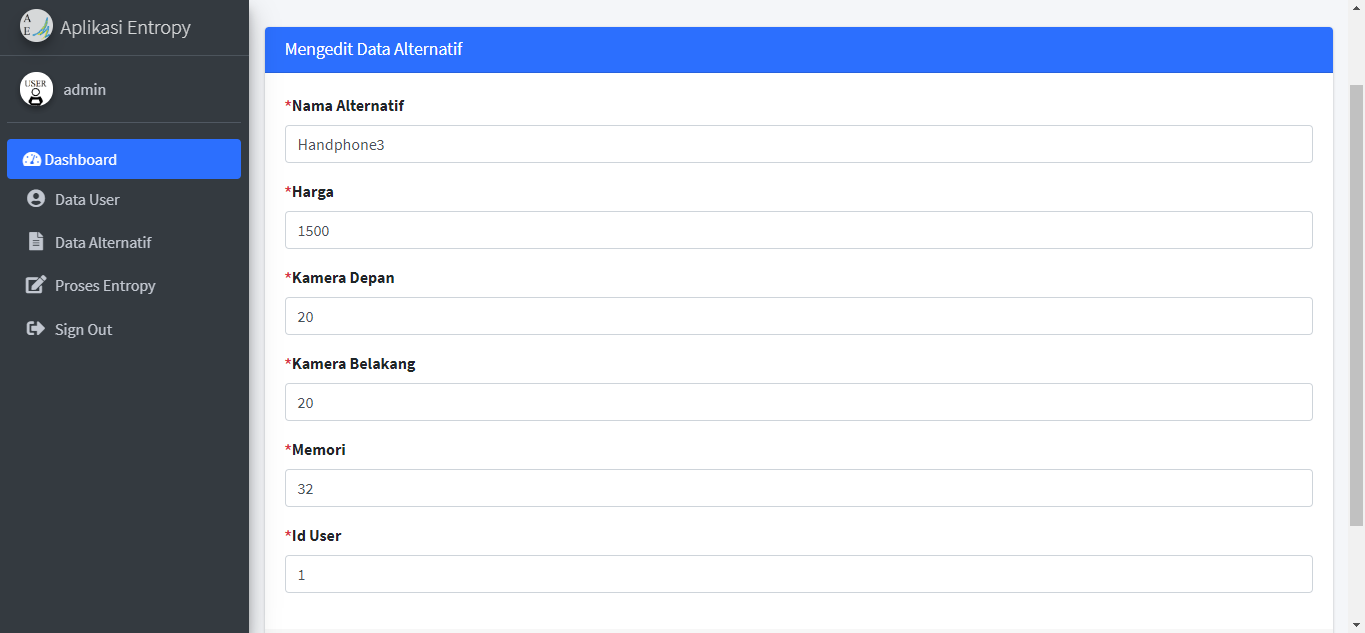
\includegraphics[width=0.90\textwidth]{figures/alte/4.png}}
	\caption{Form edit data alternatif}
	\label{al4}
\end{figure}
kemudian jika ingin melihat detail data alternatif dapad dengan cara masuk ke halaman detail data alternatif maka tampilannya seperti pada gambar \ref{al3} berikut ini.
\begin{figure}[!htbp]
	\centerline{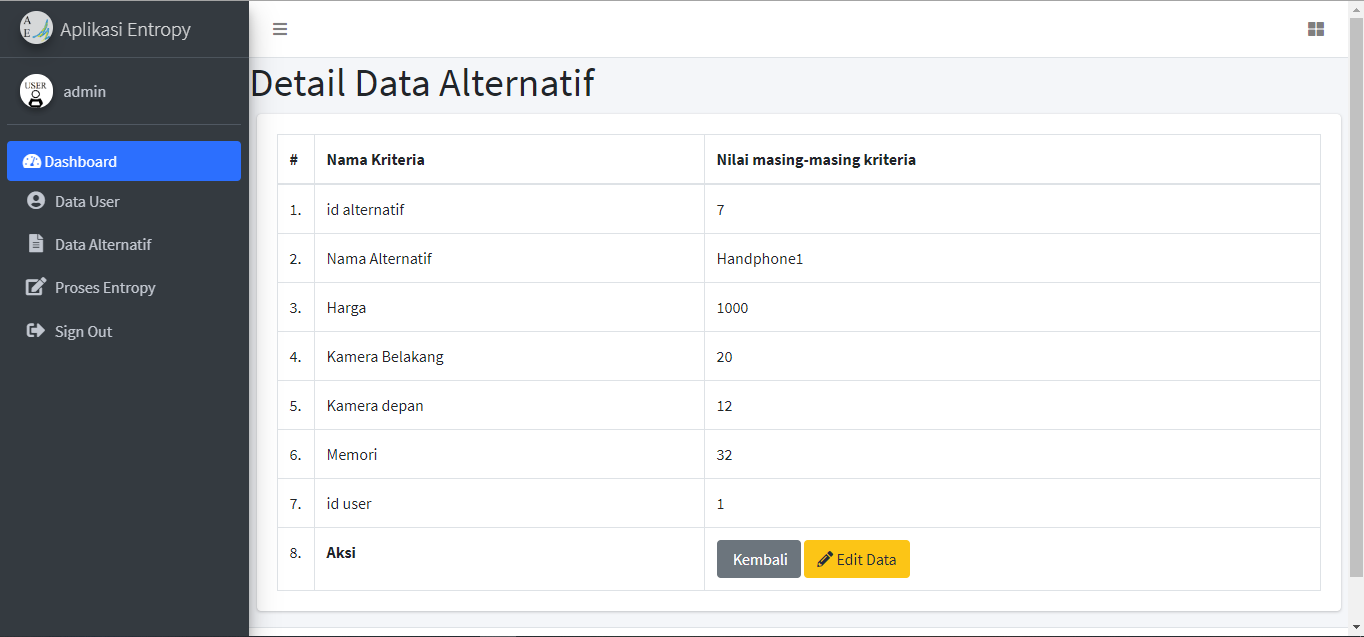
\includegraphics[width=0.90\textwidth]{figures/alte/5.png}}
	\caption{Halaman Detail data alternatif}
	\label{al5}
\end{figure}
\pagebreak
\subsection{Proses Entropy}
	kemudian jika data alternatif telah ada maka dapat di lanjutkan ke proses entropy, dimana pada proses entropy untuk admin dan selain admin berbeda, untuk admin sendiri admin harus isikan terlebih dahulu data user id pada form, untuk form nya seperti pada gambar \ref{en1} berikut:
\begin{figure}[!htbp]
	\centerline{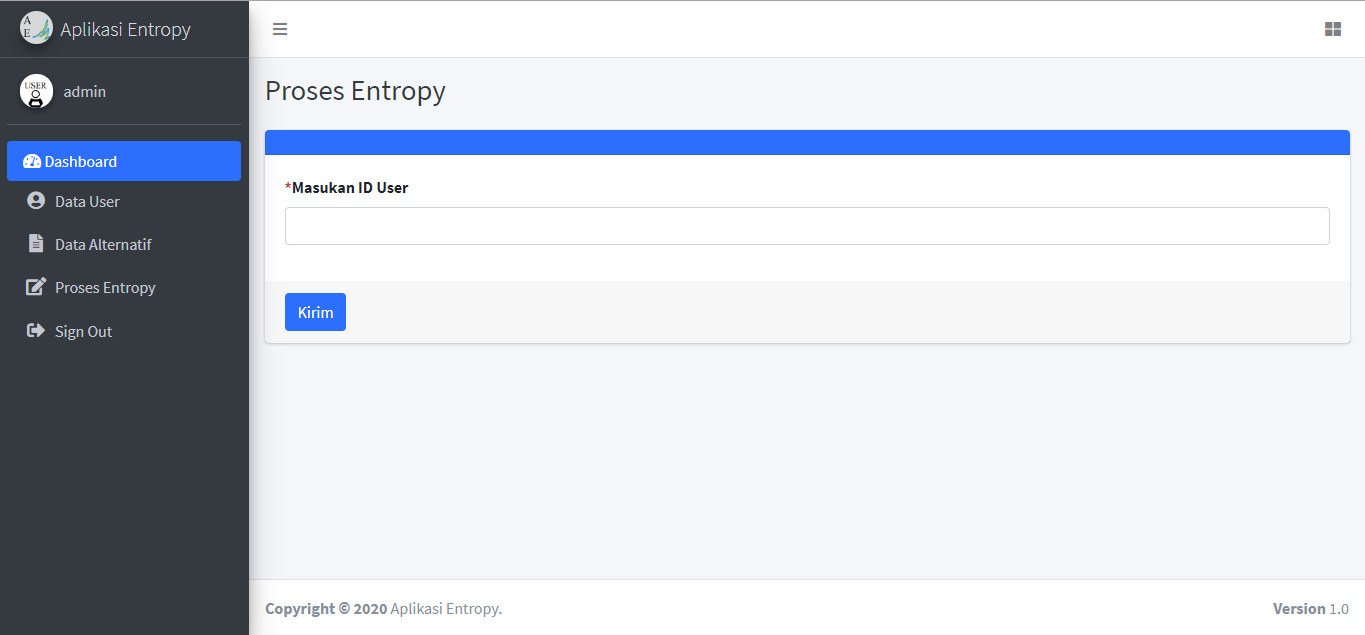
\includegraphics[width=0.90\textwidth]{figures/en/1.png}}
	\caption{Halaman insert id user}
	\label{en1}
\end{figure}

pada gambar \ref{en1} tersebut user admin memasukan id user contoh misalkan memasukan id user 1 kemudian klik kirim maka proses entropy akan berjalan kemudian untuk hasilnya seperti pada gambar \ref{en2} berikut ini
\pagebreak

kemudian pada user lain selain admin jika akan melakukan peroses entropy pada side bar tinggal menekan menu proses entropy maka proses entropy akan berjalan kemudian mendapatkan hasil seperti pada gambar \ref{en2} berikut ini.

\begin{figure}[!htbp]
	\centerline{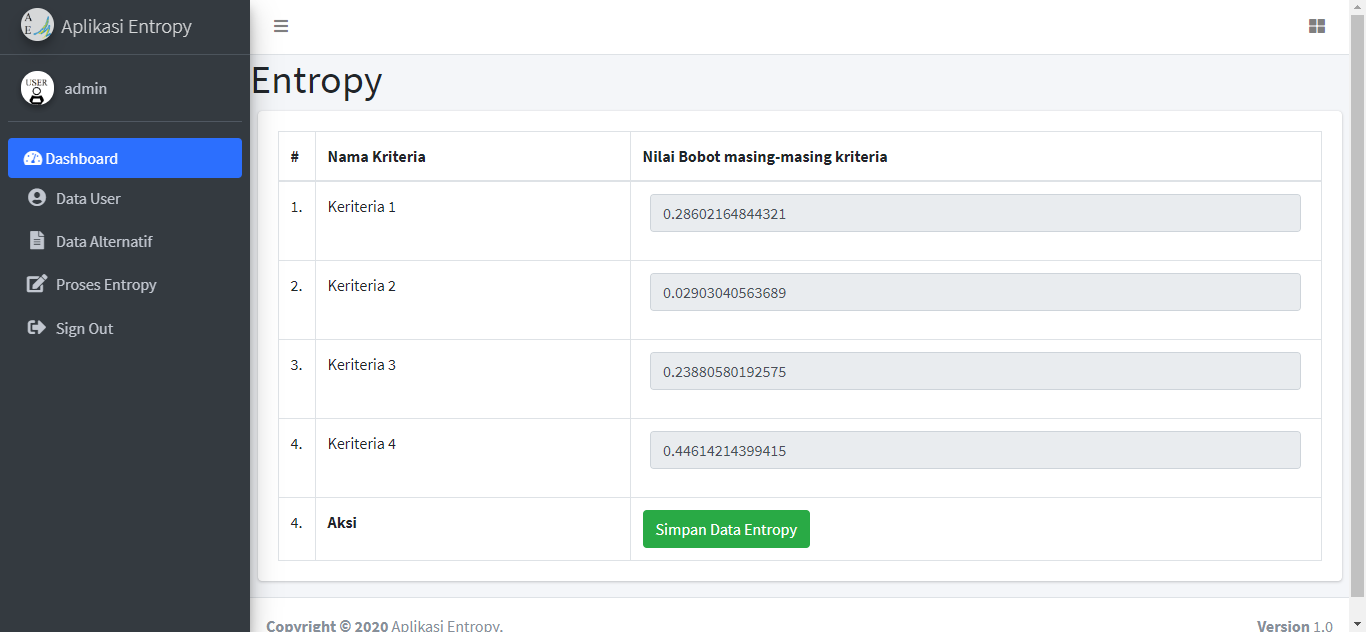
\includegraphics[width=0.90\textwidth]{figures/en/2.png}}
	\caption{Hasil Proses Entropy}
	\label{en2}
\end{figure}

jika telah muncul seperti gambar \ref{en2} kemudian langkah selanjutnya menyimpan data tersebut pada basis data sistem dengan cara menekan tombol simpan data entropy yang terdapat pada halaman tersebut.








